%------------------------------------------------------------------------------
% Template file for the submission of papers to IUCr journals in LaTeX2e
% using the iucr document class
% Copyright 1999-2013 International Union of Crystallography
% Version 1.6 (28 March 2013)
%------------------------------------------------------------------------------

\documentclass[preprint]{iucr}              % DO NOT DELETE THIS LINE
\usepackage{amssymb}
\usepackage[fleqn]{amsmath}
%\usepackage{bm}
\usepackage{graphicx}
\usepackage{tabularx}
\usepackage{booktabs}
%\usepackage{calligra}
\usepackage{longtable}
\usepackage{array}
\DeclareMathAlphabet{\mathcalligra}{T1}{calligra}{m}{n}
\def\mathbi#1{\textbf{\em #1}}
\numberwithin{equation}{section}
%\DeclareMathSymbol{\Gamma}{\mathalpha}{letters}{"00}
%\DeclareMathSymbol{\Lambda}{\mathalpha}{letters}{"03}
%\DeclareMathSymbol{\Omega}{\mathalpha}{letters}{"0A}
%\DeclareMathAlphabet{\mathitbf}{OML}{cmm}{b}{it}
\hyphenation{Niggli}
\def\mathbi#1{\textbf{\em #1}}
%\numberwithin{equation}{section}
%\DeclareMathSymbol{\Gamma}{\mathalpha}{letters}{"00}
%\DeclareMathSymbol{\Lambda}{\mathalpha}{letters}{"03}
%\DeclareMathSymbol{\Omega}{\mathalpha}{letters}{"0A}
%\DeclareMathAlphabet{\mathitbf}{OML}{cmm}{b}{it}
\usepackage{color}
%\usepackage{ulem}
\usepackage{url}
\usepackage{yfonts}
%\usepackage{xr-hyper}
%\usepackage[draft]{hyperref}
%\usepackage{bibentry}
\usepackage[normalem]{ulem}
% Redefine \underline to use \textit
\renewcommand{\underline}[1]{\textit{#1}}

\usepackage{tikz}
\usetikzlibrary{arrows.meta, positioning}
\usepackage[most]{tcolorbox}

% lca IUCr id IUCr6401
% HJB IUCr id IUCr6484
% NKS IUCr ID: IUCr7572
% lca ORCID  0000-0002-4451-1641
% HJB ORCID 0000-0002-0517-8532
% NKS ORCID 0000-0003-2786-6552


% Space macros
\usepackage{amsmath, amssymb}  % If not already included

% Crystallographic space macros
\newcommand{\HVI}{\ensuremath{\mathbf{H}^{6}}}
\newcommand{\GVI}{\ensuremath{\mathbf{G}^{6}}}
\newcommand{\SVI}{\ensuremath{\mathbf{S}^{6}}}
\newcommand{\PIII}{\ensuremath{\mathbf{P}^{3}}}
\newcommand{\FIII}{\ensuremath{\mathbf{F}^{3}}}
\newcommand{\BIV}{\ensuremath{\mathbf{B}^{4}}}
\newcommand{\CIII}{\ensuremath{\mathbf{C}^{3}}}
\newcommand{\RIII}{\ensuremath{\mathbb{R}^{3}}}

% a,b,c as base vectors of unit cells
\newcommand{\va}{\ensuremath{\mathbf{a}}}
\newcommand{\vb}{\ensuremath{\mathbf{b}}}
\newcommand{\vc}{\ensuremath{\mathbf{c}}}
\newcommand{\vd}{\ensuremath{\mathbf{d}}}



\newcommand{\vdotv}[2]{${{\bf #1 \cdot #2}}$}
\newcommand{\Imaginary}[0]{\mathcal{I}}
\newcommand{\Real}[0]{\mathcal{R}}
\newcommand{\Exchange}{\ensuremath{\mathcal{X}}}


\newcommand{\nounderline}[3]{\!\!\!\!\!\!\!\!\!#1,&\!\!\!\!\!\!\!\!\!#2,&\!\!\!\!\!\!\!\!\!#3}
\newcommand{\underlineab}[3]{\!\!\!\!\!\!\!\!\!\!\!\!\!\!\!\!\!\!\!\!\!\!\!\!\Exchange{}(#1),&\!\!\!\!\!\!\!\!\!\!\!\!\!\!\!\!\!\!\!\!\!\!\!\!\Exchange{}(#2),&\!\!\!\!\!\!\!\!\!#3}
\newcommand{\underlineac}[3]{\!\!\!\!\!\!\!\!\!\!\!\!\!\!\!\!\!\!\!\!\!\!\!\!\Exchange{}(#1),&\!\!\!\!\!\!\!\!\!\!\!\!\!\!\!\!\!\!\!\!\!\!\!\!#2,&\!\!\!\!\!\!\!\!\!\Exchange{}(#3)}
\newcommand{\underlinebc}[3]{\!\!\!\!\!\!\!\!\!\!\!\!\!\!\!\!\!\!\!\!\!\!\!\!#1,&\!\!\!\!\!\!\!\!\!\Exchange{}(#2),&\!\!\!\!\!\!\!\!\!\!\!\!\!\!\!\!\!\!\!\!\!\!\!\!\Exchange{}(#3)}

\newcommand{\scalar}[1]{\ensuremath{#1}}
\newcommand{\scalarsub}[2]{\ensuremath{#1_{#2}}}


\usepackage{makecell}
\renewcommand\cellalign{l}
\renewcommand\cellgape{\Gape[4pt]}


%-------------------------------------------------------------------------
% Information about journal to which submitted
%-------------------------------------------------------------------------
\journalcode{A}              % Indicate the journal to which submitted
%   A - Acta Crystallographica Section A
%   B - Acta Crystallographica Section B
%   C - Acta Crystallographica Section C
%   D - Acta Crystallographica Section D
%   E - Acta Crystallographica Section E
%   F - Acta Crystallographica Section F
%   J - Journal of Applied Crystallography
%   M - IUCrJ
%   S - Journal of Synchrotron Radiation
\makeatletter
\font\dummyft@=dummy \relax
\makeatother


\begin{document}                  % DO NOT DELETE THIS LINE
	
	%-------------------------------------------------------------------------
	% The introductory (header) part of the paper
	%-------------------------------------------------------------------------
	
	% The title of the paper. Use \shorttitle to indicate an abbreviated title
	% for use in running heads (you will need to uncomment it).
	
	% Authors' names and addresses. Use \cauthor for the main (contact) author.
	% Use \author for all other authors. Use \aff for authors' affiliations.
	% Use lower-case letters in square brackets to link authors to their
	% affiliations; if there is only one affiliation address, remove the [a].
	
	% Use \vita if required to give biographical details (for authors of
	% invited review papers only). Uncomment it.
	
	% lca IUCr id IUCr6401
	%\vita{Author's biography}
	
	% Keywords (required for Journal of Synchrotron Radiation only)
	% Use the \keyword macro for each word or phrase, e.g. 
	% \keyword{X-ray diffraction}\keyword{muscle}
	
	
	% PDB and NDB reference codes for structures referenced in the article and
	% deposited with the Protein Data Bank and Nucleic Acids Database (Acta
	% Crystallographica Section D). Repeat for each separate structure e.g
	% \PDBref[dethiobiotin synthetase]{1byi} \NDBref[d(G$_4$CGC$_4$)]{ad0002}
	
	%\PDBref[optional name]{refcode}
	%\NDBref[optional name]{refcode}
	
	%-------------------------------------------------------------------------
	% The introductory (header) part of the paper
	%-------------------------------------------------------------------------
	
	% The title of the paper. Use \shorttitle to indicate an abbreviated title
	% for use in running heads (you will need to uncomment it).
	\begin{center}
		{\LARGE \emph{\today}} \\
	\end{center}
	
	\title{\PIII, linearizing unit cell parameters}
	\shorttitle{properties of \PIII}
	
	% Authors' names and addresses. Use \cauthor for the main (contact) author.
	% Use \author for all other authors. Use \aff for authors' affiliations.
	% Use lower-case letters in square brackets to link authors to their
	% affiliations; if there is only one affiliation address, remove the [a].
	
	
	\cauthor[a]{Lawrence C.}{Andrews}{larry6640995@gmail.com}{}
	\author[a]{Herbert J.}{Bernstein}
	
\aff[a]{Ronin Institute for Independent Scholarship 2.0, USA}


	% Use \shortauthor to indicate an abbreviated author list for use in
	% running heads (you will need to uncomment it).
	
	\shortauthor{Andrews and Bernstein}
	
	% Use \vita if required to give biographical details (for authors of
	% invited review papers only). Uncomment it.
	
	% lca IUCr id IUCr6401
	%\vita{Author's biography}
	
	% Keywords (required for Journal of Synchrotron Radiation only)
	% Use the \keyword macro for each word or phrase, e.g. 
	% \keyword{X-ray diffraction}\keyword{muscle}
	
	\keyword{lattice}
	\keyword{unit cell}
	\keyword{polar}
	\keyword{\PIII}
	
	
	\maketitle                        % DO NOT DELETE THIS LINE

	
	
	\newcommand{\si}{\ensuremath{s_1}}
	\newcommand{\sii}{\ensuremath{s_2}}
	\newcommand{\siii}{\ensuremath{s_3}}
	\newcommand{\siv}{\ensuremath{s_4}}
	\newcommand{\sv}{\ensuremath{s_5}}
	\newcommand{\svi}{\ensuremath{s_6}}
	
	% Scalar vectors
	\newcommand{\Svec}{\ensuremath{\{ \si, \sii, \siii, \siv, \sv, \svi \}}}
	\newcommand{\SvecA}{\ensuremath{\{ -\si, -\si+\sii, \si+\siii, \si+\sv, \si+\siv, \si+\svi \}}}
	
	% Operators / maps
	\newcommand{\OPES}{\ensuremath{E^3\!\to\!S^6}}
	\newcommand{\OPESS}{
		
		\[ E^3\!\to\!S^6 \]
		
	}
	\newcommand{\MSVI}{\ensuremath{M_{S^6}}}
	\newcommand{\MEIII}{\ensuremath{M_{E^3}}}
	
	% Symbolic markers
	\newcommand{\Plus}{\ensuremath{\mathcal{P}}}
	\newcommand{\Minus}{\ensuremath{\mathcal{M}}}
	
	
	
	\begin{abstract}
		The space \PIII{} is introduced, derived from unit cell axial lengths and interaxial angles. \PIII{} enables linearization of unit cell parameters using three polar coordinate bases.

	\PIII{} serves as a compact, 
	interpretable alternative to more abstract spaces such as \GVI{} and \SVI{}.

	\end{abstract}
	% Appendices appear after the main body of the text. They are prefixed by
	% a single \appendix declaration, and are then structured just like the
	% body text.
	
	
	\section{Introduction}
	
	In crystallography, unit cell geometry is conventionally encoded in a six-dimensional parameter space 
	\ensuremath{\HVI{}=(a,b,c, \alpha, \beta, \gamma).}\footnote{``H'' was chosen to
		honor early French crystallographer Ren\'e Just Ha\"uy.} However, \HVI{} is not a metric space
	(where distances can be simply defined), nor is \HVI{} a vector space (where 
	objects can be added and subtracted). In the same sense, symmetry operations
	have no simple representations in \HVI{}. In consequence, \HVI{} has no
	simple measure of the ``difference'' between two lattices; how can one 
	compare a difference of 1 \AA{}ngstrom unit vs. one angular degree?
	
[\underline{	Note: Boris Delaunay in his later publications chose to render
	his surname as ``Delone'' (which is still pronounced the same as Delaunay).}]
	
	For the above reasons, other spaces are often used to describe lattices, often for specialized purposes; see Table  \ref{tbl_spaces}. Figure \ref{fig_spaces} shows relationships among
	several of these spaces. Although some of these spaces, such as \HVI{} and	\FIII{} are in almost daily use, they are not often referred to 
	as ``spaces''. In the case of \FIII{}, symmetry elements are linear
	operations in this space, and fractional coordinates of atomic positions
	are vectors expressed in this space.

	
We propose a ``linearized'' space, \PIII{}, derived from \HVI{}, but
having all measures in \AA{}ngstrom units (or other chosen linear measures.)

\renewcommand{\arraystretch}{1.3}

\begin{longtable}{@{}c@{\quad}l@{\quad}p{7cm}@{}}
	\caption{Crystallographic spaces with their scalar definitions and analytical purposes}
	\label{tbl_spaces} \\
	
	\toprule
	\textbf{Space} & \textbf{Scalars / Coordinates} & \textbf{Purpose} \\
	\midrule
	\endfirsthead
	
	\multicolumn{3}{@{}c@{}}{\textit{Table \thetable\ continued}} \\
	\toprule
	\textbf{Space} & \textbf{Scalars / Coordinates} & \textbf{Purpose} \\
	\midrule
	\endhead
	
	\midrule
	\multicolumn{3}{@{}c@{}}{\textit{Continued on next page}} \\
	\endfoot
	
	\bottomrule
	\endlastfoot
	
	$\HVI$ &
	\parbox[t]{5.5cm}{
		$a,\, b,\, c \in \mathbb{R}_{>0}$ — edge lengths\\
		$\alpha,\, \beta,\, \gamma \in (0^\circ, 180^\circ)$ — opposing angles\\
		
	} &
	Composite geometric parameter space $\mathbb{R}_{>0}^3 \times (0^\circ, 180^\circ)^3$. Lengths are unconstrained; angles are geometrically restricted. The angles must obey the spherical triangle inequalities (summing to less than 360 degrees, and the sum of any 2 must not exceed the third). \HVI{} is useful for conventional lattice descriptions, but limited in symmetry representation and metric-based classification. \\
	\midrule
	\FIII{} &
	$\vec{a},\, \vec{b},\, \vec{c} \in \mathbb{R}^3$ &
	Base vector space in \RIII. Coordinates are the three-space base vectors of a unit cell. Lattices are defined using the
	components of \FIII{}, and translational symmetry is described 
	in \FIII{}. \\	
	\midrule
	
	\BIV{} &
	\ensuremath{\vec{a},\, \vec{b},\, \vec{c},\, (-\vec{a}-\vec{b}-\vec{c}) \text{ in } \mathbb{R}^3} &
	Base vector space in \FIII{} plus the negative sum of the three base vectors. 
	This set of vectors is used in the definition of \SVI{}, which
	is the space of Selling/Delone reduction.\\
	\midrule

	\PIII{} &
	\parbox[t]{5.5cm}{
		$(|\vec{a}|,\alpha),\ (|\vec{b}|,\beta),\ (|\vec{c}|,\gamma)$\\
		$\Rightarrow$\\
		\hspace*{0.5cm}$(|\vec{a}|\cos\alpha,\, |\vec{a}|\sin\alpha)$\\
		\hspace*{0.5cm}$(|\vec{b}|\cos\beta,\, |\vec{b}|\sin\beta)$\\
		\hspace*{0.5cm}$(|\vec{c}|\cos\gamma,\, |\vec{c}|\sin\gamma)$\\
		also known as $(p_1, p_2, p_3)$
	} &
	Polar coordinate space defined in terms of unit cell axial
	lengths and their opposing angles (opposing, the angle between the other two unit cell axes). It is a compact and smooth alternative to $\HVI$. Useful for comparing unit cells. (This work) \\
		\midrule
	
	\SVI{} &
	\parbox[t]{5.5cm}{
		$s_1 = \vec{b} \cdot \vec{c},\, s_2 = \vec{a} \cdot \vec{c},\, s_3 = \vec{a} \cdot \vec{b}$\\
		$s_4 = \vec{a} \cdot \vec{d},\, s_5 = \vec{b} \cdot \vec{d},\, s_6 = \vec{c} \cdot \vec{d}$\\
		\quad where $\vec{d} = -\vec{a} - \vec{b} - \vec{c}$
	} &
	Used for Selling/Delone reduction. The scalar components are dot products between lattice vectors. \SVI{} supports Bravais lattice classification. 24 Bravais types were defined using the scalar components of \SVI{} by Delone (1975), later revised using \SVI{} \cite{andrews2023measuring}. \\
		\midrule
	
	\GVI{} &
	\parbox[t]{5.5cm}{
		$g_1 = \vec{a} \cdot \vec{a},\, g_2 = \vec{b} \cdot \vec{b},\, g_3 = \vec{c} \cdot \vec{c}$\\
		$g_4 = 2\vec{b} \cdot \vec{c},\, g_5 = 2\vec{c} \cdot \vec{a},\, g_6 = 2\vec{a} \cdot \vec{b}$
	} &
	\GVI{} is based on the metric tensor and used for Niggli reduction and lattice distance computation \cite{Andrews2014}. The International Tables describe 44 Bravais types using scalar expressions derived from \GVI{} \cite{ITC_VolumeA_2016}. \\
		\midrule
	
\CIII{} &
	\parbox[t]{5.5cm}{
		From \SVI{} scalars: $s_1,\dots,s_6$\\
		$c_1 = (s_1, s_4),\ c_2 = (s_2, s_5),\ c_3 = (s_3, s_6)$\\
		where the parentheses denote a complex number
	} &
	\CIII{} associates scalar pairs identified by Delone as ``opposites.'' Symmetry and Selling/Delone reduction simplify in this space \cite{andrews2023complex}. \\
		\midrule
	
	$\mathbf{DC7u}$ &
	\parbox[t]{5.5cm}{
		$d_1,\, d_2,\, d_3$ — edge lengths\\
		$d_4,\, d_5,\, d_6$ — shortest face diagonals\\
		$u$ — shortest body diagonal
	} &
	$\mathbf{DC7u}$: unsorted Dirichlet Cell space derived from Niggli-reduced cells. Defined as a 7D vector of distances. Fully invertible and smooth; used for rapid lattice distance computation \cite{bernstein2023invertible}. \\
	
\end{longtable}


\begin{figure}
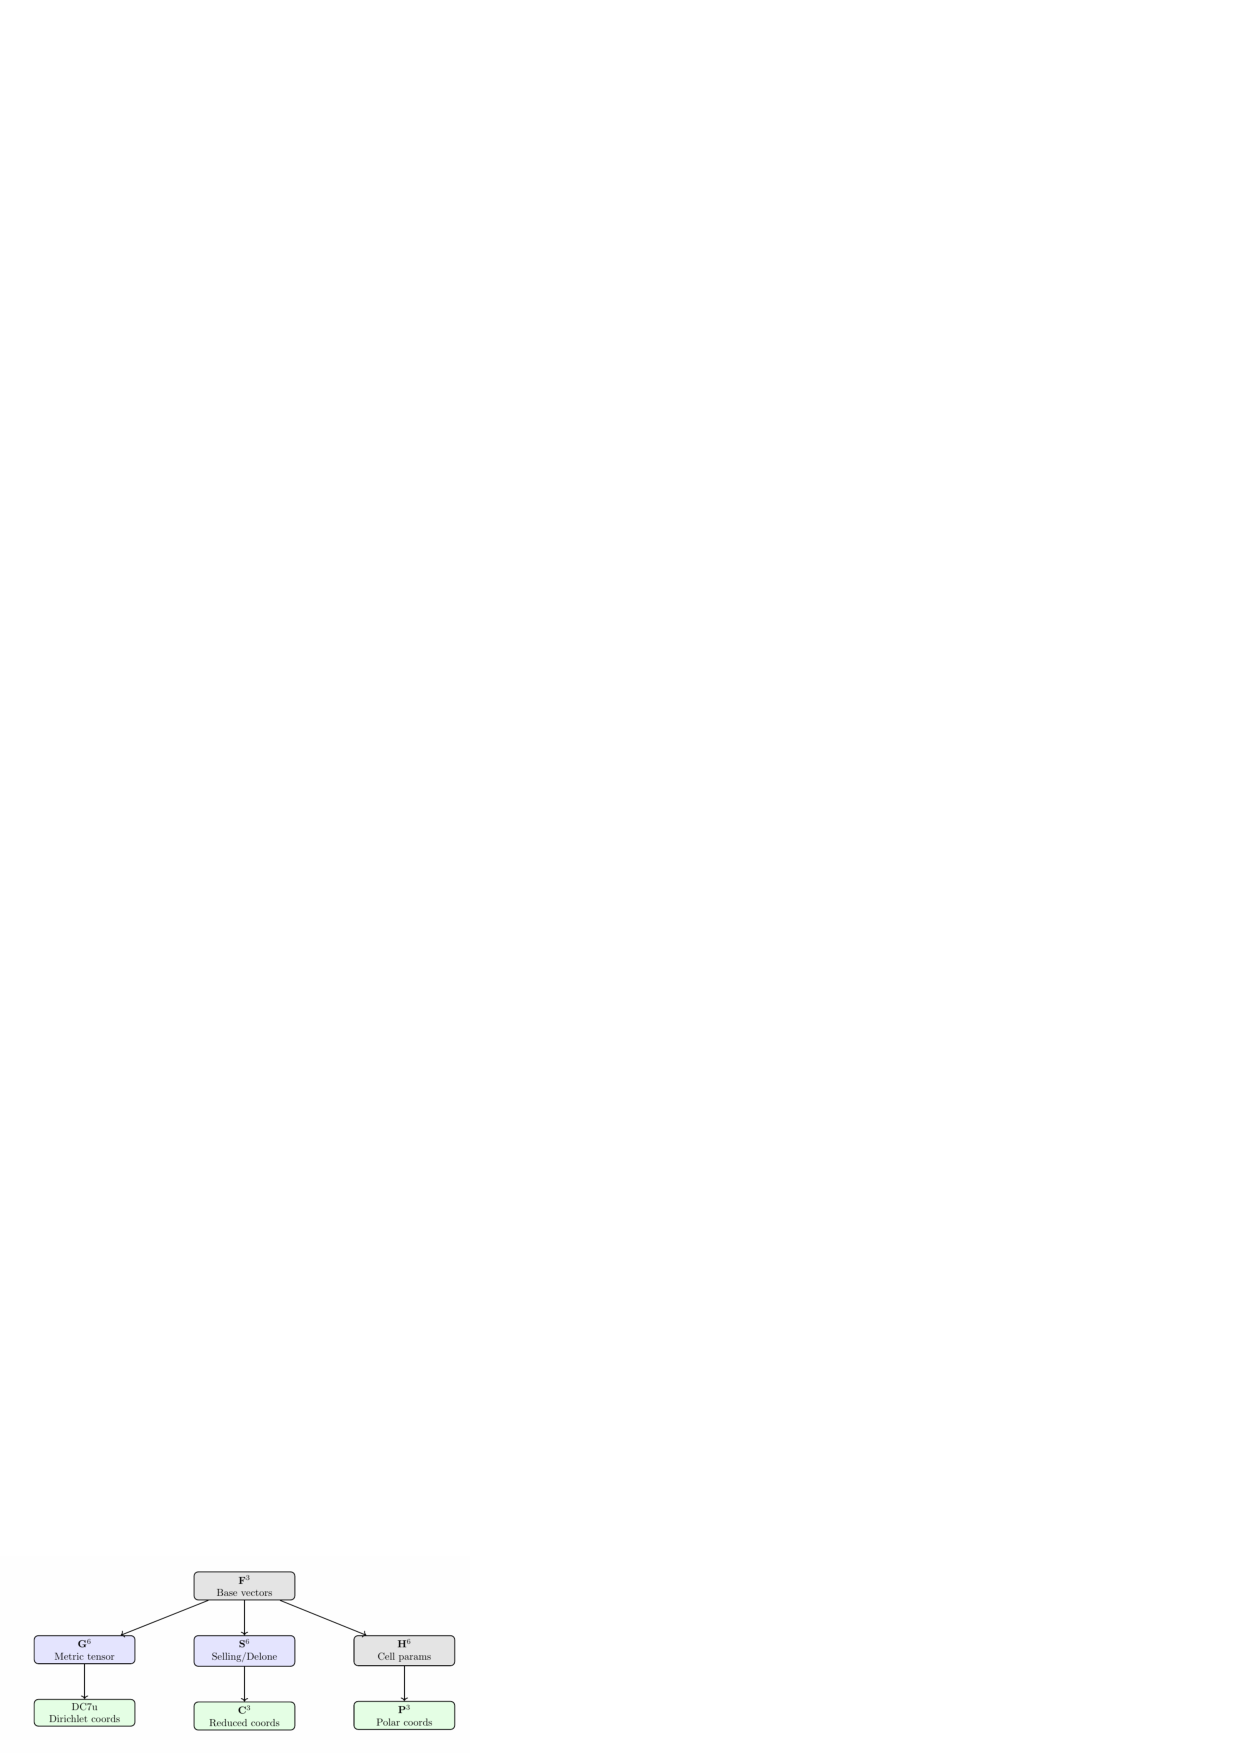
\includegraphics[]{P3_fig1.png}
\label{fig_spaces}
\caption{Schematic relationships among crystallographic spaces. The base vector 
	space \FIII{} gives rise to three scalar spaces: metric tensor space \GVI{}, 
	Selling/Delone space \SVI{}, and conventional cell parameter space \HVI{}. 
	Each transforms into a reduced or classification space: $\mathbf{DC7u}$ from \GVI{}, 
	\CIII{} from \SVI{}, and \PIII{} from \HVI{}.}
\end{figure}

\section{	\PIII{} Is introduced.}

\citeasnoun{Delone1975} repeatedly pointed out the relationship of the
``opposite'' scalars in the tetrahedron representations of the Selling
scalars. Examining those relationships shows that the opposite terms 
are pairs where a term involving $\mathbf{a}$ is opposite a term involving $\alpha$, {\it etc.}

As described in Table \ref{tbl_spaces}, the Selling scalars are a vector:
[$s_1, s_2, s_3, s_4, s_5, s_6$]. \citeasnoun{Delaunay1932} represents
their relationships as the edge components of a tetrahedron as 
shown in Figure \ref{tetrahedron}.




\begin{figure}
	\begin{center}
		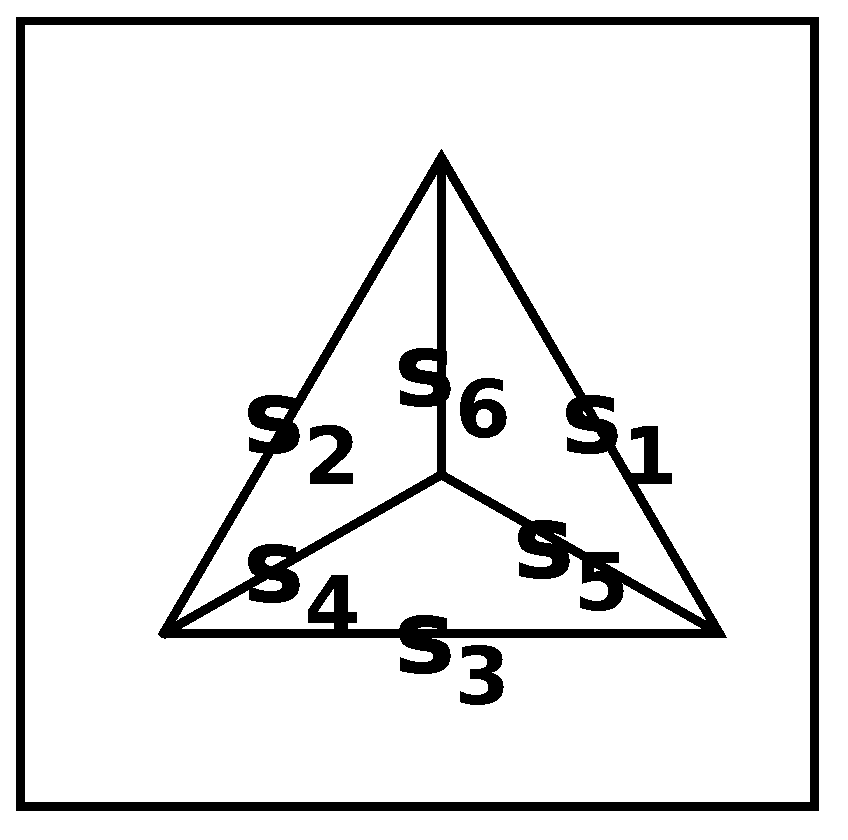
\includegraphics[width=0.3\columnwidth]{tetrahedron}
		\label{tetrahedron}
		\caption{The relationships of the Selling scalars as
		described by  \citeasnoun{Delaunay1932}, but labeled using the vector components of \SVI{} \cite{andrews2023measuring}. Visualized as a
		3 dimensional tetrahedron, scalar $s_1$ is
		opposite scalar $s_4$, etc. The number of each scalar is the 
		position in the \SVI{} vector. See Table \ref{tbl_spaces}
		for the definitions of the scalars in space \SVI{}. }

	\end{center}
\end{figure}



Extending the observation of \citeasnoun{Delone1975}, the idea occurs
to make a triple of those pairs. Since each pair has
one length and one angle, we consider each pair as the definition of
a polar coordinate. The result is \PIII{}, a space of three two-dimensional polar coordinates. See Table \ref{tbl_spaces} for the
formal description.  Two uses immediately are obvious.

The first use applies the two-dimensional character of the coordinates of \PIII{}. They
allow simple-to-plot representations of collections of unit cells. Plotting
each of the coordinates of \PIII{} generates plots that are easily
interpreted as crystallographic axial length/opposite angle pairs. The
distance of a point from the origin has a length equal to the axial length, and the interaxial
angle between the 2 other bases (plotted as the angle from the x-axis) is illustrated on the plots. Basically, together the three plots of the three coordinates are
simple projections of \HVI{}. See Section \ref{graphical}.


A second use is allowing the calculation of Euclidean distances between
pairs of unit cells. Because \PIII{} can be represented as three xy planes, the Euclidean difference between
any two unit cells described as \PIII{} can be easily computed. This use
contrasts with \HVI{}, where incommensurate lengths and angles do not
lend themselves to a distance calculation. See Section \ref{comparing}.



\section{Relationship to Other Spaces}

While \PIII{} is derived from the same foundational cell parameters as $\mathbf{H^6}$, $\mathbf{P^3}$ sidesteps issues of angular nonlinearity  that arise in the conventional cell representation. Compared with $\mathbf{C^3}$ \cite{andrews2023complex}, which derives coordinates from $\mathbf{S^6}$, the construction of $\mathbf{P^3}$ is more geometric than algebraic. It provides a useful intermediary: more interpretable than metric tensors or other spaces, but less abstract than \SVI{} or \GVI{}.

	

	
\section{Graphical display of projections}{
\label{graphical}
\PIII{}
allows simple-to-plot representations of collections of unit cells. 
See Figures \ref{PlotPolar_raw}, \ref{PlotPolar_Niggli}, and  \ref{PlotPolar_Delone}, where 100 randomly chosen triclinic cells are plotted
(Figure \ref{PlotPolar_raw}), and the effects of unit cell reduction
are demonstrated (Figure \ref{PlotPolar_Niggli} and Figure \ref{PlotPolar_Delone} ).
}


\begin{figure}
    \begin{center}
	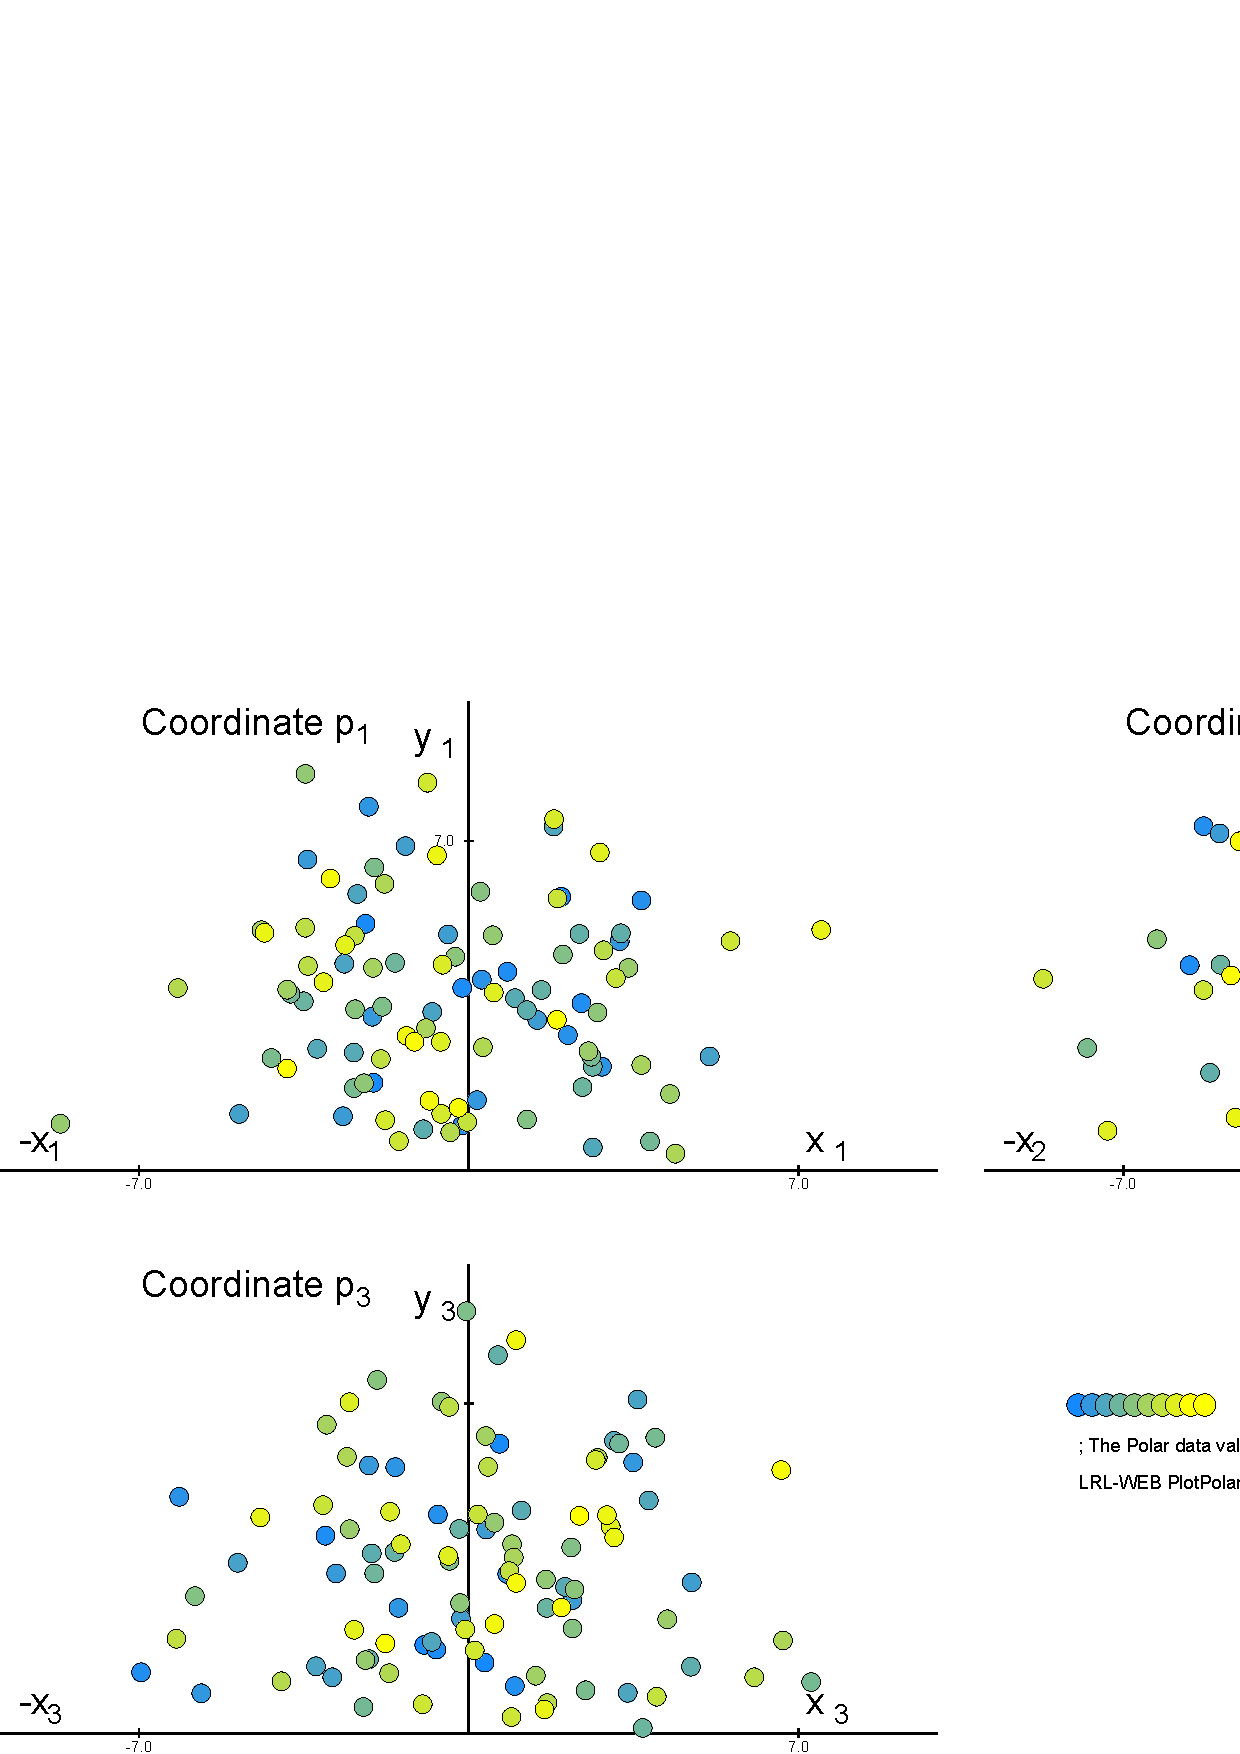
\includegraphics[width=\columnwidth]{PlotPolar_raw.png}
	\label{PlotPolar_raw}
	\caption{Scatter plots of 100 randomly selected
		 primitive triclinic unit cells represented in \PIII{}. Each of the 3 components of \PIII{}
		 is shown. (Colors reflect the order of input of the unit cells.)}
	\end{center}
\end{figure}

\begin{figure}
    \begin{center}
	\includegraphics[width=\columnwidth]{PlotPolar_Niggli.png}
	\label{PlotPolar_Niggli}
	\caption{The same 100 randomly selected primitive triclinic unit cells shown in Figure \ref{PlotPolar_raw}, Niggli-reduced}.
	\end{center}
\end{figure}


\begin{figure}
	\begin{center}
	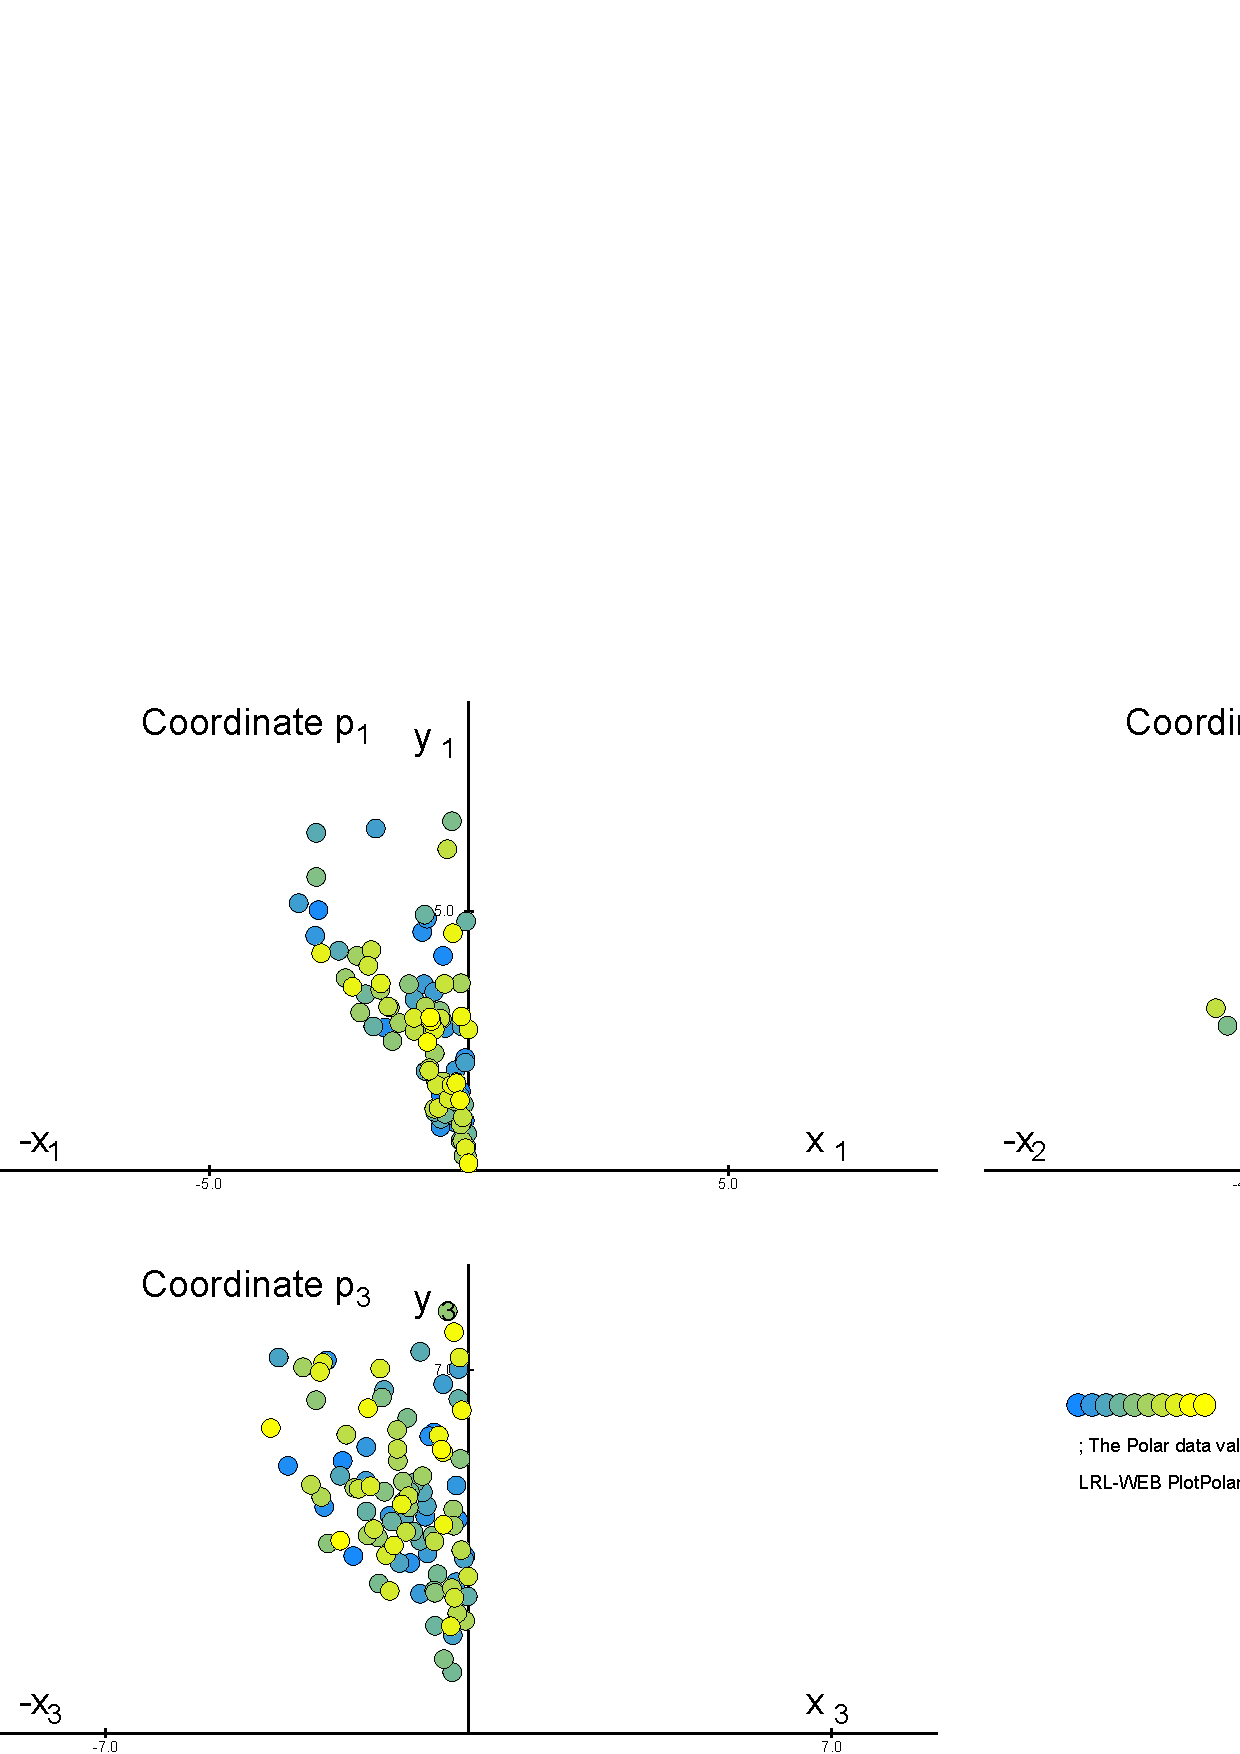
\includegraphics[width=\columnwidth]{PlotPolar_Delone.png}
	\label{PlotPolar_Delone}
	\caption{Scatter plots of 100 randomly selected
		primitive triclinic unit cells represented in \PIII{} as shown in Figure \ref{PlotPolar_raw}, Selling /Delone-reduced}.
	\end{center}
\end{figure}

\section{Comparing different unit cells}
\label{comparing}

In 3-space, measuring the Euclidean distance between two points is just computing the square root
of the sum of the squares of the differences in the three coordinates. Similarly in \PIII{},
we compute distances from the square root of the sum of squared differences between the three
polar coordinates. Polar coordinates have a Euclidean measure from
their xy representation. So, taking the 6 scalar values of 2 unit cells
presented in \PIII{}, we calculate a Euclidean distance by the ordinary
method. 



Let us compare two cells derived by modifying a primitive unit cell to form two slightly modified cells, one by changing $\gamma$, and one by changing $\vec{c}$.
\begin{enumerate}
	\item P 10 10 10  90 90 90
	\item P 10 10 10  90 90 91
	\item P 10 10 10.1  90 90 90
\end{enumerate}
The Euclidean distances between these cells are:
\begin{itemize}
	\item 1--2: 0.175
	\item 1--3: 0.100
	\item 2--3: 0.202
\end{itemize}

In this example, a 1.0$^\circ$ change in $\gamma$ yields a Euclidean distance comparable to a 0.1~\AA{} change in the $c$-axis length.

	
	\section{Summary}
	
	The space \PIII{} is introduced. Less abstract than spaces based
	on dot products and metric tensors, it provides a simple way to understand the
	method for comparing unit cells and a convenient method of displaying 
	unit cells.
	
	
	
	
	\section{Availability of code} CmdToP3 and PlotPolar are available in github.com, in
	\url{https://github.com/duck10/LatticeRepLib.git}.
	
	%\appendix
	
	
	\ack{{\bf Acknowledgements}}

Careful copy-editing and corrections by Frances C. Bernstein are 
gratefully acknowledged. 

	\ack{{\bf Funding information}}      
	
	Funding for this research was provided in part by:  
	U.S. Department of Energy Offices of Biological and 
	Environmental Research and of Basic Energy Sciences 
	(grant No. DE-AC02-98CH10886; grant No. E-SC0012704); 
	U.S. National Institutes of Health (grant No. P41RR012408; 
	grant No. P41GM103473; grant No. P41GM111244; 
	grant No. R01GM117126,
	grant No. 1R21GM129570); Dectris, Ltd.
	
	\section{Synopsis}
	
	\PIII{} is a linearized description of unit cell parameters,
	created from the usual lengths and angles of the unit cell. It 
	provides a useful metric for comparing unit cells and a
	convenient base for displaying and comparing unit cells.
	
	\bibliography{Reduced}
	
	\bibliographystyle{iucr}
	
	
	
	%-------------------------------------------------------------------------
	% TABLES AND FIGURES SHOULD BE INSERTED AFTER THE MAIN BODY OF THE TEXT
	%-------------------------------------------------------------------------
	
	% Simple tables should use the tabular environment according to this
	% model
	
	% Postscript figures can be included with multiple figure blocks
	
	%C:\Users\lca\Source\Repos\LatticeRepLib\x64\Debug>plotc3
	%; Graphical output SVG file =PLT__2023-03-07.13_43_35.svg
	%
	%C:\Users\lca\Source\Repos\LatticeRepLib\x64\Debug>cmdniggli | plotc3
	%; Graphical output SVG file =PLT__2023-03-07.13_44_06.svg
	%
	%C:\Users\lca\Source\Repos\LatticeRepLib\x64\Debug>cmddelone | plotc3
	%; Graphical output SVG file =PLT__2023-03-08.07_11_03.svg
	%
	%C:\Users\lca\Source\Repos\LatticeRepLib\x64\Debug>cmdniggli | cmdperturb 5 20 | plotc3
	%; Graphical output SVG file =PLT__2023-03-08.09_00_13.svg
	%
	%C:\Users\lca\Source\Repos\LatticeRepLib\x64\Debug>cmdniggli | cmdperturb 5 100 | plotc3
	%; Graphical output SVG file =PLT__2023-03-08.09_00_21.svg
	
\end{document}                    % DO NOT DELETE THIS LINE
%%%%%%%%%%%%%%%%%%%%%%%%%%%%%%%%%%%%%%%%%%%%%%%%%%%%%%%%%%%%%%%%%%%%%%%%%%%%%%
